\chapter{Исследовательский раздел}
В данном разделе приведены характеристики устройства, на котором проводилось измерение времени работы программного обеспечение, результаты проведенных замеров.

\section{Технические характеристики}
Технические характеристики используемого устройства:
\begin{itemize}
    \item[---] операционная система --- Ubuntu Linux x86\_64~\cite{Ubuntu};
    \item[---] память --- 16 Гб;
    \item[---] процессор --- AMD Ryzen 5 5500U (6x2.10 ГГц)~\cite{AMD}.
\end{itemize}

\section{Замеры времени}
Время обрисовки затерялось на компьютере с указанными техническими характеристиками и использованием библиотеки \textit{<ctime>}~\cite{ctime}. Были проведены замеры времени отрисовки одного кадра в зависимости от количества точек задаваемой пользователем кривой и времени отрисовки одного кадра в зависимости от числа разбиений окружности при построении тела.

На рисунке~\ref{fig:poly} приведены  результаты замеров времени отрисовки одного кадра в зависимости от числа разбиений окружности при построении тела вращения. Для каждого числа разбиений время посчитано как среднее от 100 проведенных замеров. Замеры проводились при фиксированном количестве точек кривой.

\begin{figure}[H]
	\centering
	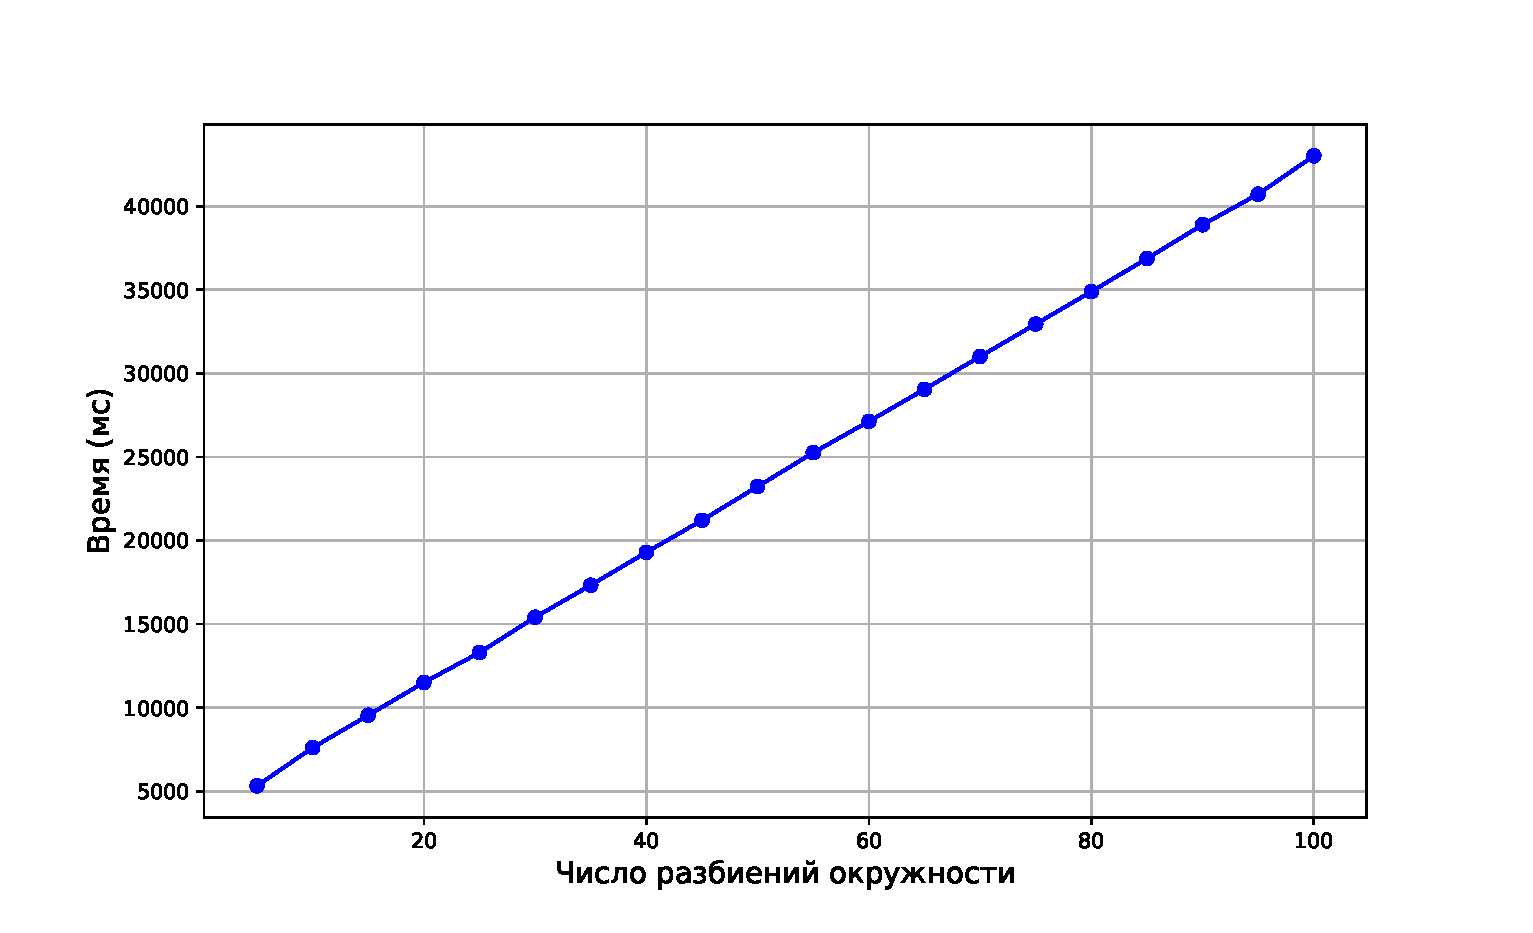
\includegraphics[scale=0.6]{img/graph_poly.eps}
	\caption{Зависимость времени отрисовки одного кадра от числа разбиений окружности}
	\label{fig:poly}
\end{figure}

На рисунке~\ref{fig:curve} приведены  результаты замеров времени отрисовки одного кадра в зависимости от количества точек кривой. Для каждого числа точек время посчитано как среднее от 100 проведенных замеров. Замеры проводились при фиксированном числе разбиений окружности.

\begin{figure}[H]
	\centering
	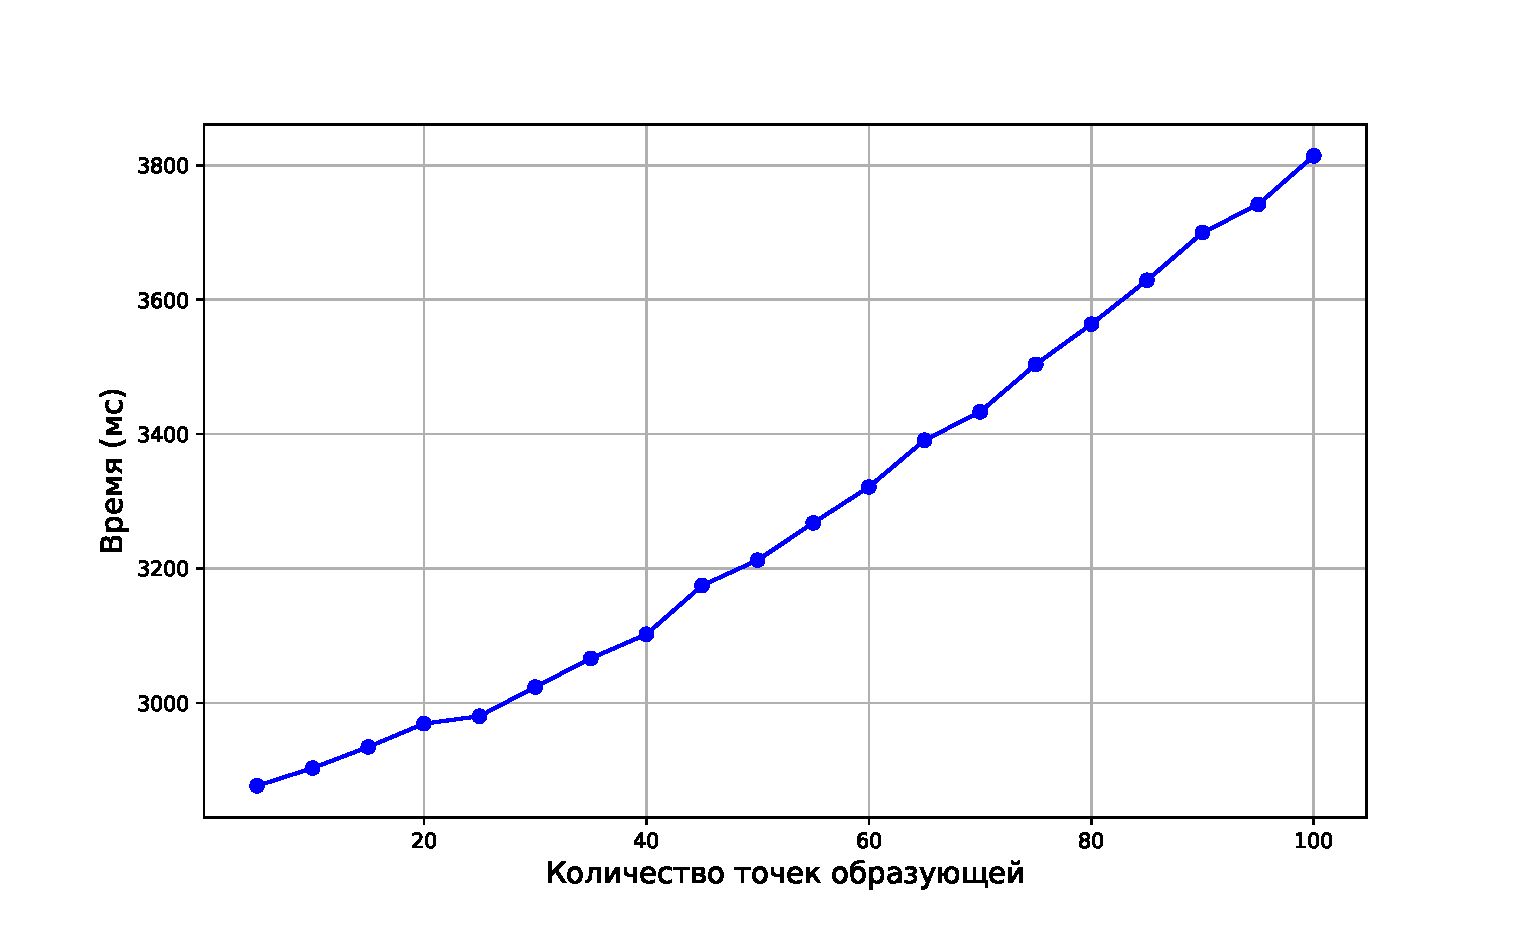
\includegraphics[scale=0.6]{img/graph_curve.eps}
	\caption{Зависимость времени отрисовки одного кадра от количества точек кривой}
	\label{fig:curve}
\end{figure}

В результате исследования была получено, что зависимость времени отрисовки кадра от числа разбиений окружности и количества точек кривой линейна. Такая зависимость наблюдается вследствие пропорционального увеличения количества треугольников в модели, которые необходимо обработать, при увеличении данных параметров.


\textbf{ВЫВОД}

В данном разделе приведены результаты работы программного обеспечения и результаты исследования. Результаты исследования совпали с ожидаемыми, так как время отрисовки сцены прямо пропорционально числу разбиений окружности и количеству точек кривой. 
\clearpage